
%%%%%%%%%%%%%%%%%%%%%%%%%%%%%%%%%%%%%%%%%%%%%%%%%%%%%%%%%%%%%%%%%%%%%%%%%
%           Capítulo 3: Diseño e implemantacion                         %
%%%%%%%%%%%%%%%%%%%%%%%%%%%%%%%%%%%%%%%%%%%%%%%%%%%%%%%%%%%%%%%%%%%%%%%%%

\chapter{Diseño del experimento}

El desarrollo de la aplicación considera las siguientes situaciones para considerar un sistema útil para el manejo de almacenes. Dentro de las características útiles menciono los siguientes puntos.

\begin{numerate}
\item Registro de usuario
\item Modificación de Almacenes
\item Modelamiento de productos
\end{numerate}

Entre las características principales de un sistema de gestión de almacenes están los siguientes puntos.

\begin{numerate}
\item Códigos de barras
\item Herramientas de informes
\item Previsión de inventarios
\item Alertas de inventarios
\end{numerate}

%%%%%%%%%%%%%%%%%%%%%%%%%%%%%%%%%%%%%%%%%%%%%%%%%%%%%%%%%%%%%%%%%%%%%%%%%
%                          Modelamiento de Almacenes                    %
%%%%%%%%%%%%%%%%%%%%%%%%%%%%%%%%%%%%%%%%%%%%%%%%%%%%%%%%%%%%%%%%%%%%%%%%%
\section{Modelamiento de los almacenes}

Dentro de un contexto variado de empresa, lo normal es dividirlas en dos grupos, que son empresas dedicadas a la fabricación y empresas dedicadas al comercio. De estos dos grupos de empresas, la gestión de almacenes es diferente. La gestión de almacenes en empresas dedicadas a la fabricación debe de considerarse un flujo interno que describa los movimientos de los materiales internamente para su transformación. Sin embargo tanto para la empresa dedicada a la fabricación de productos como a una empresa dedicada al comercio, ambos tienes que gestionar almacenes para la venta; en el caso de la primera esta gestión será para los productos terminados y una empresa comercial, le interesará la gestión de sus mercaderías a la venta.\\

En el siguiente listado muestro un resumen de las necesidades para una empresa de fabricación y una dedicada al comercio. [\citep{PCD:2019:Online}]

\begin{numerate}
\item PARA FABRICACIÓN
\begin{numerate}
    \item Seguimiento de materiales
    \item Niveles de inventario para piezas y productos terminados
    \item Reordenación automática
    \item Integración ERP
\end{numerate}
\item PARA ALMACENES
 \begin{numerate}
    \item Sistema de códigos de barras avanzado (QR, y demás)
    \item Soporte a ubicación múltiple
    \item Sistema de seguimiento de estantería
    \item Soporte de selección de pedidos
\end{numerate}
\end{numerate}

Cabe aclarar que el listado anterior no implica una necesidad en cada una de los tipos de empresas ya que cada empresa puede prescindir de alguna de ellas, claro que esto también implicaría un costo asociado.

%%%%%%%%%%%%%%%%%%%%%%%%%%%%%%%%%%%%%%%%%%%%%%%%%%%%%%%%%%%%%%%%%%%%%%%%%
%                          Modelado                                     %
%%%%%%%%%%%%%%%%%%%%%%%%%%%%%%%%%%%%%%%%%%%%%%%%%%%%%%%%%%%%%%%%%%%%%%%%%
\section{Modelamiento de usuario}

El funcionamiento de sistemas en línea, el usuario es el elemento por donde la aplicación funciona. Si bien no se está creando un sistema de gestión de usuarios, se debe modelar un correcto uso de recursos en función al usuario.\\

Un sistema en línea, debe proveer las opciones para que un usuario cualquiera pueda acceder a él. Para tal efecto es importante crear mecanismos de registro, con validación para que el usuario pueda registrarse y acceder a sus recursos.\\

El registro no debe ser complejo ni tomar mucho tiempo. Desde este punto de vista, el usuario debe registrar sus datos básicos, como ser su nombre y su correo electrónico. Estos datos son almacenado y además es importante que el usuario ingrese una clave de acceso, la que llamaremos “Password”. Muchos sistemas, realizan comprobaciones para que el “Password” de usuario sea lo más seguro, tanto para el usuario como para el sistema mismo.\\

De los detalles anteriores, se deriva los siguientes diagramas que modelan el usuario en el sistema.

\begin{figure}
  \centering
    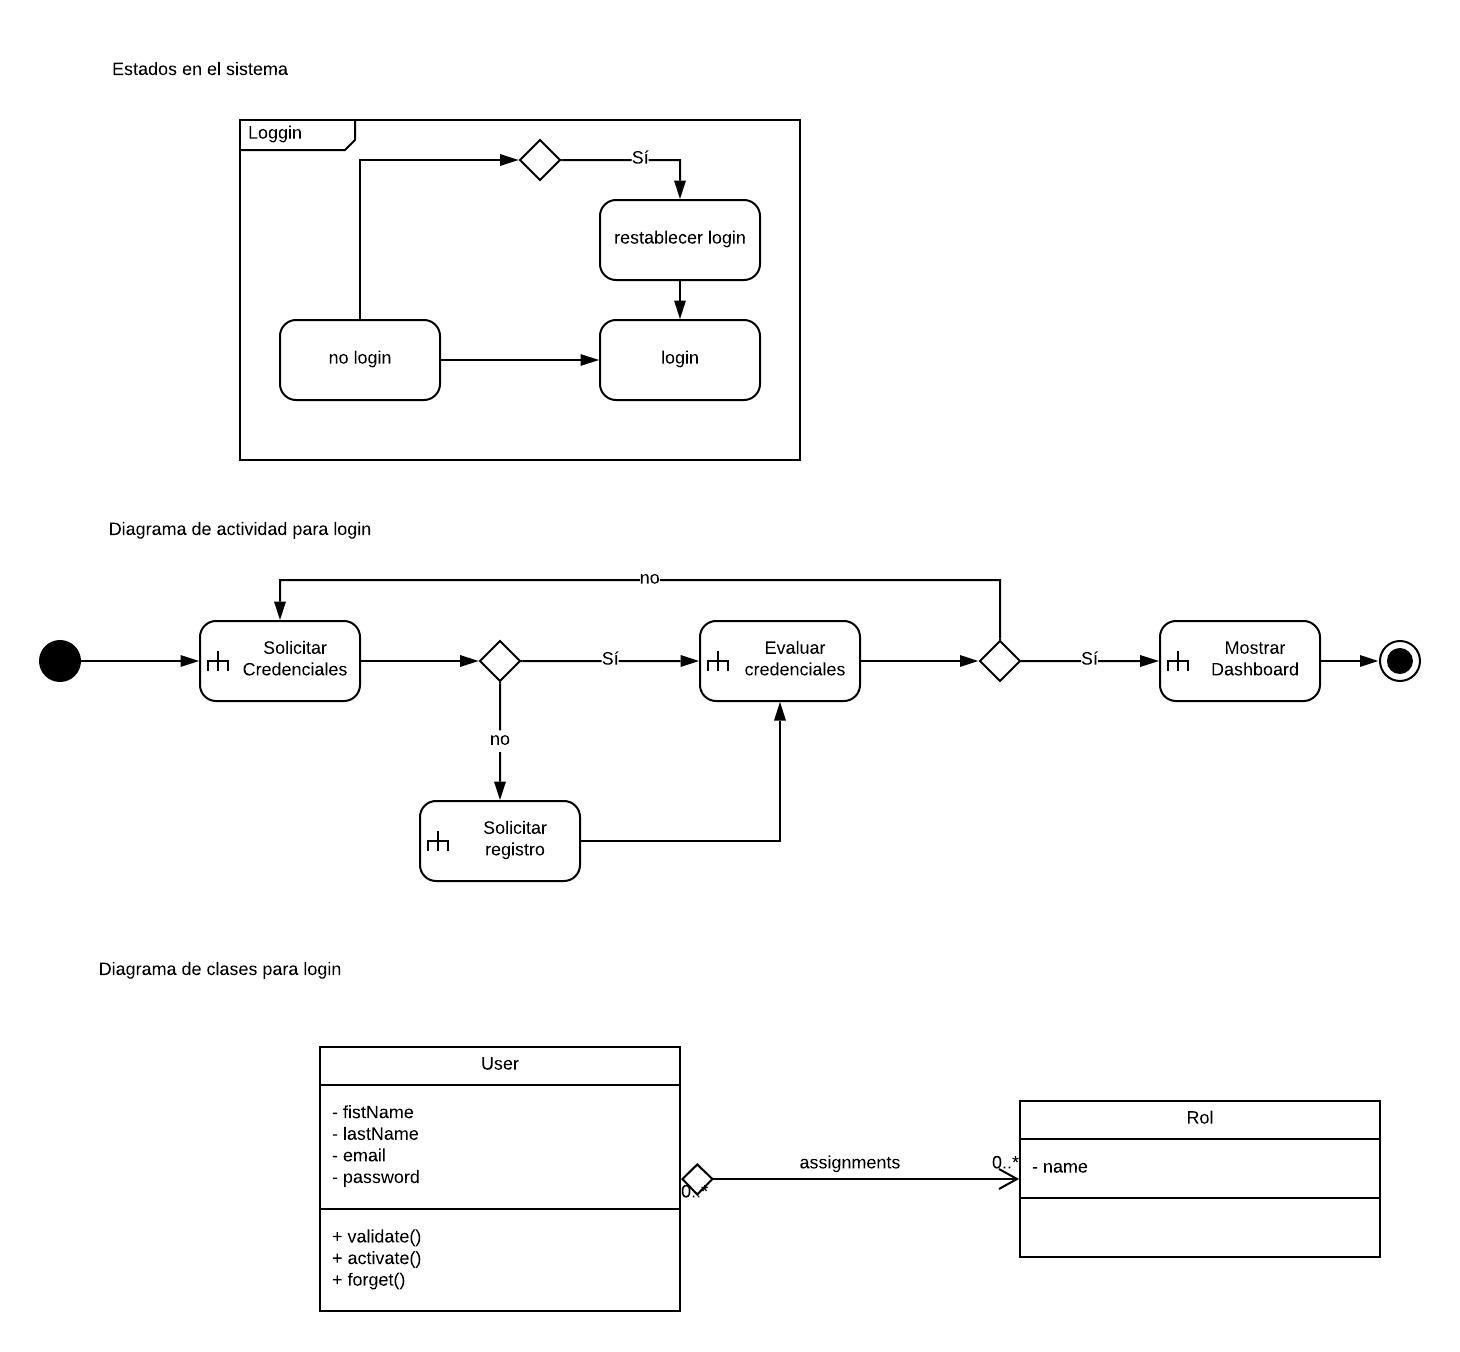
\includegraphics[scale=0.7]{./Capitulo3/figs/ADDStock-user-login.jpeg}
  \caption{Diagrama de estados, diagrama de actividades y diagrama de clases para el modelamiento de usuarios en el sistema de gestión de almacenes.}
  \label{user_login}
\end{figure}

El funcionamiento de manejo de usuarios en el sistema, se basa en el concepto de roles, lo cual permite al sistema manejar opciones. La división por roles nos permite definir accesos a diferentes opciones en el sistema. Para el propósito del sistema de gestión de almacenes, lo importante es permitir al usuario mismo, proteger su información de usuarios con menos privilegios que están encargados de tareas más concretas dentro de un sistema de almacenes.\\

La estructura de roles básicos que se puede manejar en el sistema son los siguientes:

\begin{itemize}
\item Superadmin
\item Admin
\item User
\begin{itemize}
    \item Vendedor
    \item Almacenero
\end{itemize}
\end{itemize}

El listado anterior muestra una estructura básica, ya que la idea es permitir al usuario crear más usuarios con roles que el mismo usuario pueda definir y por lo tanto los accesos que puedan tener a los recursos que vaya creando el usuario.\\

Se ha tomado pequeñas funciones que todos los sistemas de usuarios manejan y son la recuperación de “Password” de usuario y la mantención de sesión.

\section{Modelamiento de la empresa}

El sistema define la existencia de una empresa con cada cuenta de usuario. De este modo, se tiene una restricción de una empresa por cuenta creada. Sin embargo cada empresa puede tener definido varios usuarios, por lo cual haremos uso de los roles para definir una cuenta principal, que estará a cargo de la empresa y de los usuarios de esta misma.\\

El modelamiento general estará basado en una sola clase, que guardará la información de la empresa.\\

\begin{figure}
  \centering
    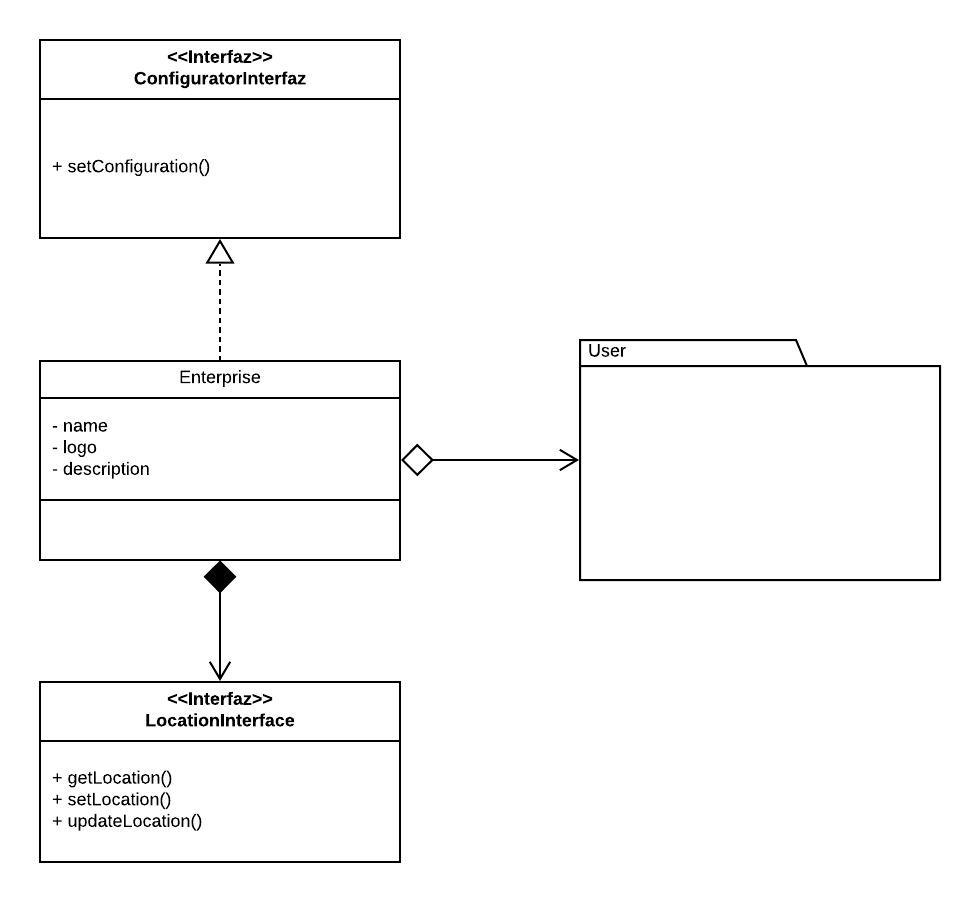
\includegraphics[scale=0.9]{./Capitulo3/figs/ADDStock-enterprise.jpeg}
  \caption{Diagrama de clases para el modelamiento de empresa.}
  \label{enterprise}
\end{figure}

La definición de empresa se basa en la información que se requiere guardar y esencialmente se trata del nombre de la empresa y su dirección. Cabe mencionar que la información tiene que ser guardada y está íntimamente ligada a las configuraciones que haya a realizarse en la aplicación.\\

En el modelo (figura \ref{enterprise}) presentado se trata de especificar que el objeto empresa interviene en las configuraciones que se realizarán en la aplicación. Mediante el objeto empresa se realizará las configuraciones en la aplicación.\\

Este modelo mostrado en \ref{enterprise} requiere una explicación de porqué se está usando una interface para la localización. La idea general de localización está muy ligada a los almacenes, ya que se puede definir sucursales, puntos de donde los proveedores se encuentren y varios productos pueden estar en distintos lugares para su almacenado.

\section{Modelando el producto}

El producto es el tema principal de la aplicación y la información circulara en función a los productos que se tengan almacenados, en proceso. Incluso los productos que sean considerados de distinta manera, como por ejemplo los materiales, suministros. Estos a su vez pueden tener un grado más de especialización ya que pueden ser materiales de transformación, materiales de uso como son los consumibles.\\

En este modelamiento todavía no se tomará en cuenta los movimientos de productos en almacenes ni su almacenamiento propiamente dicho.\\

La necesidad de información que hasta ahora se ha modelado corresponde a la figura \ref{Product-classes}

\begin{figure}
  \centering
    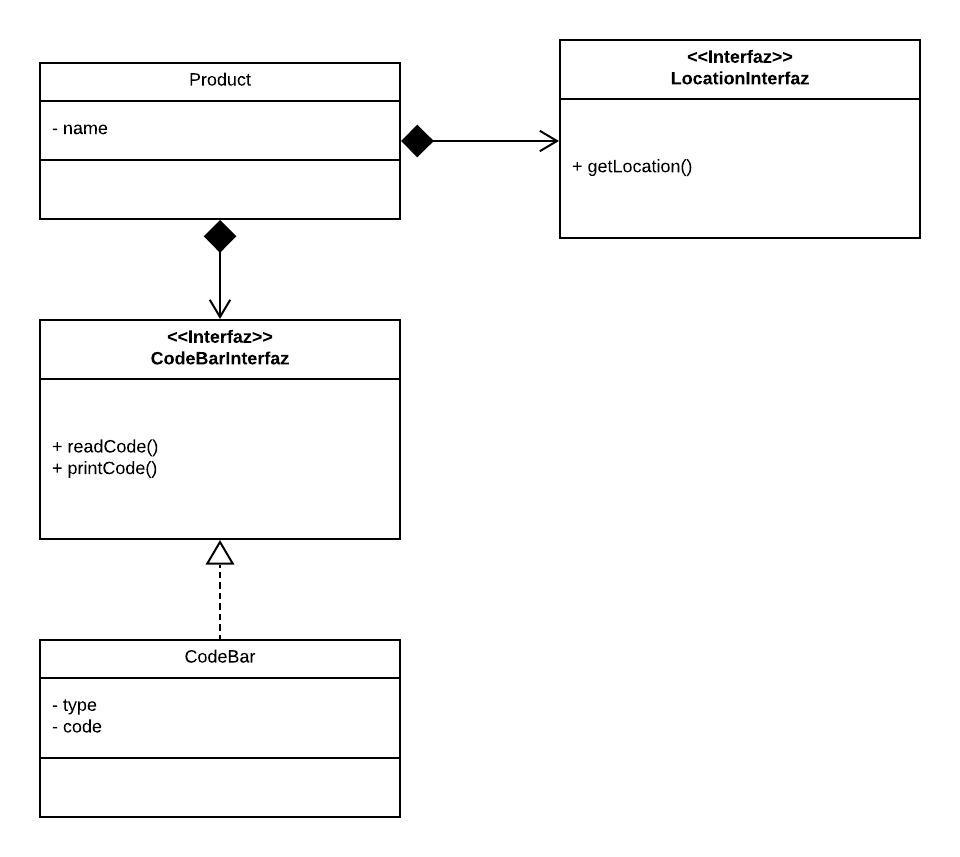
\includegraphics[scale=0.9]{./Capitulo3/figs/ADDStock-Product.jpeg}
  \caption{Diagrama de clases para el modelamiento de producto.}
  \label{Product-classes}
\end{figure}